\chapter{Неравенства, оценки и методы доказательства}\label{chap:c17}\markright{Глава 19}
\section{Что значит оценить величину}
Ранее неравенства чаще появлялись как условия для неизвестного. Теперь цель меняется: не обязательно найти точное значение выражения, иногда достаточно доказать, что оно не выходит за нужные границы. Все числовые переменные этой главы действительные, если отдельно не сказано, что они целые или натуральные.

\begin{definition}
\term{Верхняя оценка} (upper bound) величины \(F\) — число или выражение \(M\), для которого при всех оговорённых условиях выполнено \(F\le M\). \term{Нижняя оценка} (lower bound) задаётся неравенством \(m\le F\). Вместе они дают \(m\le F\le M\).
\end{definition}
\begin{definition}
\term{Случай равенства} (equality case) в неравенстве — допустимые значения переменных, при которых обе его стороны равны. Оценку \(F\le M\) называют \term{достижимой} (attainable), если хотя бы при одном допустимом выборе получается \(F=M\).
\end{definition}
Для \(0\le x\le10\) равенство
\[
x(10-x)=25-(x-5)^2
\]
даёт \(x(10-x)\le25\). Граница достигается при \(x=5\), поэтому это наибольшее значение выражения. Число \(30\) тоже является верхней оценкой, но не наибольшим значением. Нельзя доказывать оптимальность границы только тем, что она подходит: нужен также допустимый пример, на котором она достигается.

\par\addvspace{5pt}\begin{lrbox}{\CatFlowBox}\begin{minipage}[t]{\linewidth}
\setlength{\parskip}{5pt}\setlength{\columnsep}{4.5mm}\setlength{\intextsep}{0pt}
\begin{wrapfigure}[9]{r}{54mm}
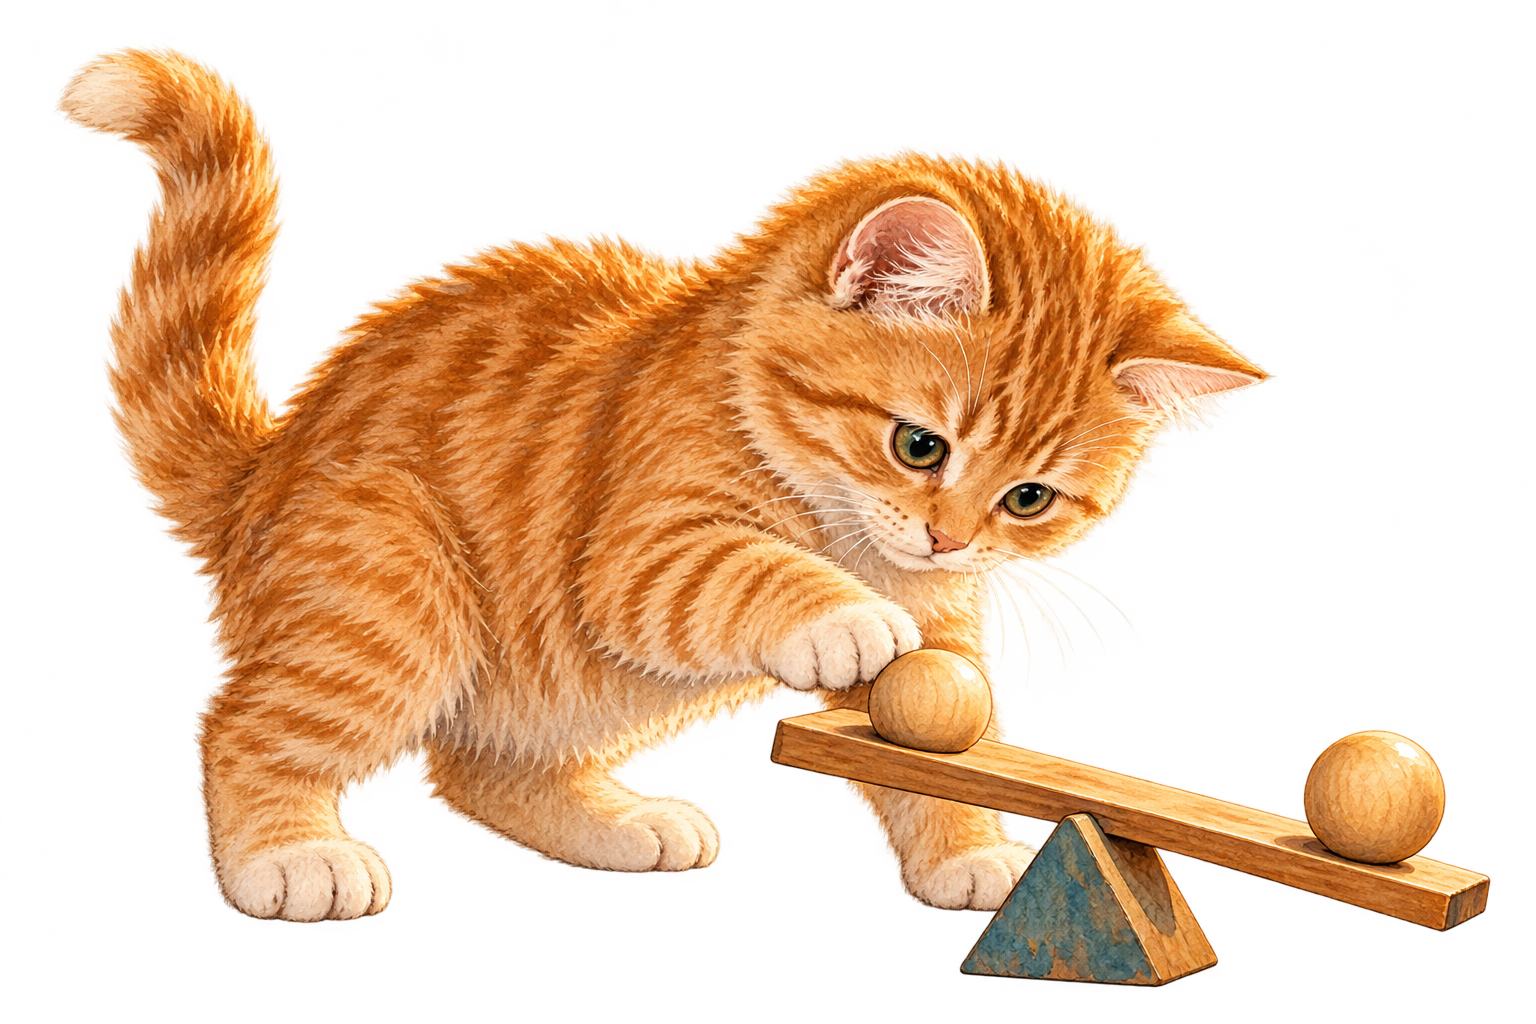
\includegraphics[width=54mm,height=58mm,keepaspectratio]{images/unique/art-43.png}
\label{catflow:43}
\end{wrapfigure}
Работа с оценками начинается с внимательного чтения условий. Нужно понять, какие значения могут принимать переменные, какие из них зависят друг от друга и какие действия допустимы. Затем полезно заранее представить случай равенства: он подсказывает, какую разность превращать в квадрат или какие два неотрицательных выражения сравнивать. После получения границы надо вернуться к исходным условиям и проверить, существует ли указанный случай равенства. Например, в задаче о длинах нельзя использовать отрицательную сторону, а в задаче о количестве предметов нельзя выбирать дробное число предметов. Такая проверка связывает вычисление с его смыслом и предотвращает ситуацию, когда формально найденная граница недостижима. Оценка остаётся полезной и тогда, когда точное значение неизвестно: она может гарантировать достаточный запас материала, ограничить ошибку измерения или показать, что нужный результат вообще невозможен.
\par\WFclear\end{minipage}\end{lrbox}%
\ifdim\dimexpr\ht\CatFlowBox+\dp\CatFlowBox\relax<64mm\dp\CatFlowBox=\dimexpr64mm-\ht\CatFlowBox\relax\fi%
\noindent\usebox{\CatFlowBox}\par\addvspace{5pt}
\section{Знаки, квадраты и цепочки оценок}
Прибавлять одно и то же число к обеим частям неравенства можно без изменения его направления. Умножение на положительное число сохраняет направление, на отрицательное — меняет его, а умножение на ноль уничтожает информацию о строгом порядке. Поэтому перед делением на выражение нужно установить, что оно ненулевое, и определить его знак.

Например, из \(x^2\ge x\) нельзя безусловно получить \(x\ge1\) делением на \(x\). При \(x<0\) знак изменится, а при \(x=0\) деление невозможно. Разложение \(x(x-1)\ge0\) сразу даёт все решения: \(x\le0\) или \(x\ge1\).

Из \(A\le B\) и \(B\le C\) следует \(A\le C\). Если требуется \(A=C\), должны одновременно выполняться равенства во всех звеньях этой цепочки. Для положительных \(0<a\le b\) также \(\frac1a\ge\frac1b\): это получается делением \(a\le b\) на положительное \(ab\).

\begin{theorem}[Базовая оценка через квадрат]\label{thm:legacy-c17-1}
Для любых действительных \(a,b\)
\[
2ab\le a^2+b^2.
\]
Равенство выполняется тогда и только тогда, когда \(a=b\).
\end{theorem}
\begin{proof}
Разность правой и левой частей равна \(a^2+b^2-2ab=(a-b)^2\). Квадрат неотрицателен и равен нулю ровно при \(a-b=0\).
\end{proof}
Например, \(x^2+9\ge6x\) для любого \(x\); равенство возможно только при \(x=3\). Чтобы сравнивать квадраты с самими числами, нужно учитывать знак: из \(A^2\le B^2\) следует \(|A|\le|B|\), а вывод \(A\le B\) без дополнительных условий может быть неверен.

\section{Два средних и задачи на оптимальное значение}
\begin{definition}
\term{Среднее арифметическое} (arithmetic mean) чисел \(a,b\) равно \(\frac{a+b}{2}\). Для \(a,b\ge0\) их \term{среднее геометрическое} (geometric mean) равно \(\sqrt{ab}\).
\end{definition}
\begin{theorem}[Неравенство средних для двух чисел; AM--GM]\label{thm:legacy-c17-2}
Если \(a,b\ge0\), то
\[
\sqrt{ab}\le\frac{a+b}{2}.
\]
Равенство выполняется тогда и только тогда, когда \(a=b\).
\end{theorem}
\begin{proof}
Квадрат \((\sqrt a-\sqrt b)^2\) неотрицателен. Раскрывая его, получаем \(a+b-2\sqrt{ab}\ge0\). Деление на \(2\) даёт оценку. Равенство эквивалентно \(\sqrt a=\sqrt b\), то есть \(a=b\).
\end{proof}
При фиксированной сумме \(a+b=s\), где \(a,b\ge0\), отсюда
\[
ab\le\frac{s^2}{4}.
\]
Обе стороны перед возведением в квадрат неотрицательны. Граница достигается при \(a=b=\frac s2\). Так, среди прямоугольников заданного положительного периметра наибольшую площадь имеет квадрат: сумма двух соседних сторон фиксирована, а площадь равна их произведению.

Другой пример: для \(x>0\) числа \(x\) и \(\frac9x\) положительны, а их произведение равно \(9\). Поэтому \(x+\frac9x\ge6\). Равенство требует \(x=\frac9x\), откуда с учётом \(x>0\) получаем \(x=3\). Здесь неравенство даёт нижнюю границу, а допустимый выбор показывает, что она является минимумом.

\Needspace{12\baselineskip}\section{Неравенство Коши--Буняковского в двух координатах}
\begin{theorem}[Коши--Буняковский; Cauchy--Schwarz inequality]\label{thm:legacy-c17-3}
Для любых действительных \(a,b,c,d\)
\[
|ac+bd|\le\sqrt{a^2+b^2}\,\sqrt{c^2+d^2}.
\]
Равенство выполняется тогда и только тогда, когда \(ad=bc\).
\end{theorem}
\par\addvspace{5pt}\begin{lrbox}{\CatFlowBox}\begin{minipage}[t]{\linewidth}
\setlength{\parskip}{5pt}\setlength{\columnsep}{4.5mm}\setlength{\intextsep}{0pt}
\begin{wrapfigure}[13]{r}{54mm}

\includegraphics[width=54mm,height=58mm,keepaspectratio]{images/unique/art-67.png}
\label{catflow:67}
\end{wrapfigure}
\textit{Доказательство.} Раскрытие скобок даёт тождество
\[
(a^2+b^2)(c^2+d^2)-(ac+bd)^2=(ad-bc)^2\ge0.
\]
Значит, квадрат левой стороны исходного неравенства не больше квадрата правой. Обе стороны неотрицательны, поэтому можно извлечь квадратный корень. Равенство соответствует нулю \((ad-bc)^2\), то есть условию \(ad=bc\), в том числе когда одна пара координат нулевая.\hfill\(\blacksquare\)
\par\WFclear\end{minipage}\end{lrbox}%
\ifdim\dimexpr\ht\CatFlowBox+\dp\CatFlowBox\relax<64mm\dp\CatFlowBox=\dimexpr64mm-\ht\CatFlowBox\relax\fi%
\noindent\usebox{\CatFlowBox}\par\addvspace{5pt}

Например, для любых \(x,y\)
\[
|2x-3y|\le\sqrt{13}\,\sqrt{x^2+y^2}.
\]
Если \(x^2+y^2=1\), выражение \(2x-3y\) лежит между \(-\sqrt{13}\) и \(\sqrt{13}\). Верхняя граница достигается при \((x;y)=(\frac2{\sqrt{13}};-\frac3{\sqrt{13}})\), нижняя — при противоположной паре. Эта оценка станет геометрической после введения векторов.

\section{Бернулли: общая оценка вместо длинного вычисления}
\begin{theorem}[Неравенство Бернулли; Bernoulli's inequality]\label{thm:legacy-c17-4}
Для действительного \(t\ge-1\) и натурального \(n\)
\[
(1+t)^n\ge1+nt.
\]
При \(n=1\) всегда получается равенство. При \(n\ge2\) равенство выполняется ровно при \(t=0\).
\end{theorem}
\begin{proof}
База \(n=1\) — равенство. Предположим оценку для \(n\). Поскольку \(1+t\ge0\), умножение сохраняет направление:
\[
(1+t)^{n+1}\ge(1+nt)(1+t)=1+(n+1)t+nt^2\ge1+(n+1)t.
\]
Индукция доказывает утверждение. При \(t=0\) обе части равны единице. Если \(t\ne0\), то \(nt^2>0\), поэтому каждый переход к показателю \(n+1\ge2\) даёт строгое неравенство. Это доказывает и описание равенства.
\end{proof}
Например, \((1+\frac1{50})^5\ge1+\frac5{50}=\frac{11}{10}\). Это нижняя оценка, а не точный результат. Для \(t>0\) и \(n\ge2\) она строгая: сложные проценты дают больше, чем прибавление одного и того же процента только от начальной суммы.

\section{Контрпример и принцип Дирихле}
\begin{definition}
\term{Контрпример} (counterexample) к утверждению «для всех допустимых значений верно \(P\)» — один допустимый выбор, при котором \(P\) ложно. Контрпример должен удовлетворять всем условиям проверяемого утверждения.
\end{definition}
Чтобы опровергнуть \(\sqrt{a+b}\ge\sqrt a+\sqrt b\) при \(a,b\ge0\), достаточно взять \(a=b=1\): тогда \(\sqrt2<2\). Проверка ещё ста случаев для доказательства всеобщего утверждения, напротив, не годится. Полезно сначала проверить нули, отрицательные значения, границы области и возможные нулевые знаменатели: это помогает обнаружить неверную формулировку до попытки её доказать.

\begin{theorem}[Принцип Дирихле; pigeonhole principle]\label{thm:legacy-c17-5}
Пусть \(k\) — натуральное число, \(m\in\mathbb N_0\). Если не менее \(km+1\) предметов распределены по \(k\) группам, хотя бы в одной группе не менее \(m+1\) предметов.
\end{theorem}
\begin{proof}
Если бы в каждой группе находилось не более \(m\) предметов, общее число не превосходило бы \(km\). Это противоречит наличию как минимум \(km+1\) предметов. Значит, группа с требуемым количеством существует.
\end{proof}
Группы не обязательно являются физическими коробками. Это могут быть месяцы рождения, варианты ответа, дни недели или классы чётных и нечётных чисел. Каждый предмет должен попасть ровно в одну из указанных групп. Например, среди \(13\) человек найдутся двое с одним месяцем рождения, потому что месяцев \(12\). Принцип гарантирует существование совпадения, но не указывает, какой именно месяц встретится дважды.

\section{Инварианты, убывающая величина и конечный экстремум}
\begin{definition}
\term{Инвариант} (invariant) процесса — величина или свойство, сохраняющееся после каждого разрешённого шага. \term{Полуинвариант} (monovariant) — величина, которая на каждом шаге изменяется только в одном направлении: не возрастает либо не убывает. Для доказательства завершения обычно нужна более сильная проверка, чем одна монотонность.
\end{definition}
Если пару целых чисел заменяют по правилу \((a;b)\mapsto(a+1;b-1)\), сумма остаётся равной \(a+b\). Поэтому из \((8;5)\) невозможно получить \((7;7)\): суммы различаются. Если целое число изменяют на \(2\), сохраняется его чётность. Для невозможности достаточно одного различающего инварианта; совпадение найденного инварианта ещё не доказывает достижимость.

\par\addvspace{5pt}\begin{lrbox}{\CatFlowBox}\begin{minipage}[t]{\linewidth}
\setlength{\parskip}{5pt}\setlength{\columnsep}{4.5mm}\setlength{\intextsep}{0pt}
\begin{wrapfigure}[13]{l}{54mm}

\includegraphics[width=54mm,height=58mm,keepaspectratio]{images/unique/art-44.png}
\label{catflow:44}
\end{wrapfigure}
Выбор инварианта начинается с разбора одного разрешённого действия. Нужно проследить, что происходит с суммой, разностью, чётностью или числом объектов, а затем проверить сохранение для каждого допустимого вида шага. После этого утверждение распространяется на любое конечное число шагов: после первого шага свойство сохраняется, после второго сохраняется снова, и так далее. Если начальное и желаемое состояния различаются по найденному признаку, никакая последовательность действий не поможет. Обратный вывод требует осторожности: одинаковая сумма двух состояний лишь снимает одно препятствие, но не строит путь между ними. При поиске завершающего алгоритма, напротив, полезно искать величину, которая не сохраняется, а обязательно уменьшается. Чтобы исключить бесконечный процесс, надо дополнительно понять, насколько она уменьшается и где её нижняя граница.
\par\WFclear\end{minipage}\end{lrbox}%
\ifdim\dimexpr\ht\CatFlowBox+\dp\CatFlowBox\relax<64mm\dp\CatFlowBox=\dimexpr64mm-\ht\CatFlowBox\relax\fi%
\noindent\usebox{\CatFlowBox}\par\addvspace{5pt}
\begin{theorem}[Завершение по целочисленному полуинварианту]\label{thm:legacy-c17-6}
Если на каждом разрешённом шаге неотрицательная целочисленная величина \(M\) уменьшается хотя бы на \(1\), процесс содержит не более \(M_0\) шагов, где \(M_0\) — её начальное значение.
\end{theorem}
\begin{proof}
После \(s\) шагов имеем \(M\le M_0-s\); это доказывается индукцией по числу шагов. Но \(M\ge0\), значит, \(s\le M_0\). Большее число шагов невозможно.
\end{proof}
Одного строгого убывания действительных чисел недостаточно: последовательность \(1,\frac12,\frac14,\ldots\) убывает бесконечно. Здесь нет уменьшения хотя бы на фиксированную положительную величину.

\begin{definition}
\term{Наибольший элемент} (maximum) непустого множества \(A\subseteq\mathbb R\) — принадлежащее ему число \(M\), для которого \(a\le M\) при всех \(a\in A\). \term{Наименьший элемент} (minimum) определяется неравенствами \(m\le a\). Принадлежность множеству обязательна.
\end{definition}
\begin{theorem}[Экстремальные элементы конечного множества]\label{thm:legacy-c17-7}
Любое конечное непустое множество действительных чисел имеет наибольший и наименьший элементы.
\end{theorem}
\begin{proof}
Для одного элемента утверждение очевидно. Предположим, что для \(n\) элементов наибольшее число \(M\) найдено. После добавления числа \(b\) наибольшим станет \(M\), если \(b\le M\), и \(b\), если \(b>M\). Индукция доказывает существование максимума. Аналогично при добавлении числа сравнивают его с уже найденным минимумом.
\end{proof}
\term{Метод экстремального элемента} (extremal principle) состоит в выборе наибольшего или наименьшего объекта конечного набора и использовании его отличительного свойства. Для бесконечного множества вывод требует новых условий: интервал \((0;1)\) ограничен, но не имеет максимума, поскольку вместе с \(x\) содержит большее число \(\frac{x+1}{2}\). Его супремум равен \(1\), однако \(1\) интервалу не принадлежит. Именно различие между достижимым максимумом и точной верхней гранью важно при дальнейшем изучении анализа.


\section{Среднее арифметическое и геометрическое трёх чисел}
\begin{theorem}[AM–GM для трёх чисел]
Для \(a,b,c\ge0\) выполнено \(a+b+c\ge3\sqrt[3]{abc}\), причём равенство достигается тогда и только тогда, когда \(a=b=c\).
\end{theorem}
\begin{proof}Положим \(x=\sqrt[3]a,y=\sqrt[3]b,z=\sqrt[3]c\). Тождество
\[
x^3+y^3+z^3-3xyz=\tfrac12(x+y+z)\bigl((x-y)^2+(y-z)^2+(z-x)^2\bigr)
\]
даёт неотрицательность левой части. Если \(x+y+z=0\), все три числа нулевые. Иначе равенство возможно ровно при \(x=y=z\). Это равносильно \(a=b=c\).\end{proof}

\par\addvspace{2pt}\begin{lrbox}{\CatFlowBox}\begin{minipage}[t]{\linewidth}
\setlength{\parskip}{2pt}\setlength{\columnsep}{4.5mm}\setlength{\intextsep}{0pt}
\begin{wrapfigure}[12]{r}{54mm}

\includegraphics[width=54mm,height=58mm,keepaspectratio]{images/unique/art-266.png}
\label{catflow:266}
\end{wrapfigure}
Экстремальная задача на целые числа обычно содержит две разные части. Сначала доказывают, что меньшее или большее значение невозможно, затем предъявляют набор, на котором граница достигается. Неравенство без конструкции даёт лишь оценку. Конструкция без оценки показывает только один допустимый результат. Для сумм различных натуральных чисел полезно упорядочить числа: каждый следующий элемент обязан быть не меньше предыдущего плюс единица. Если добавляется условие на сумму цифр, его сначала переводят в сравнение по модулю, а потом проверяют совместимость с этой нижней границей. В ответе необходимо сохранить и различность, и натуральность, и исходное ограничение на цифры.
\par\WFclear\end{minipage}\end{lrbox}%
\ifdim\dimexpr\ht\CatFlowBox+\dp\CatFlowBox\relax<60mm\dp\CatFlowBox=\dimexpr60mm-\ht\CatFlowBox\relax\fi%
\noindent\usebox{\CatFlowBox}\par\addvspace{2pt}
\relax
\section{Оценка должна сопровождаться конструкцией}
В дискретной задаче полезно отдельно доказать, что лучшего результата быть не может, и построить допустимый пример на найденной границе. Эти два рассуждения решают разные части задачи. Условие на общую сумму ещё не гарантирует, что доступны все нужные отдельные суммы.
\begin{example}[Как доказать отсутствие пропусков]\label{ex:review-ege-c17-1}
Есть четыре монеты по \(2\) и пять монет по \(5\). Сколько монет по \(1\) надо добавить, чтобы можно было набрать каждую целую сумму от \(1\) до \(35\)? Старые монеты дают всего \(33\), поэтому единичных нужно не менее двух.
Двух достаточно. С помощью четырёх двоек и двух единиц получаются все целые суммы от \(0\) до \(10\): интервалы \([2j;2j+2]\), \(j=0,\ldots,4\), перекрываются в концах. После добавления \(k\) пятёрок получаем все суммы в \([5k;5k+10]\), \(k=0,\ldots,5\). Соседние интервалы тоже перекрываются; их объединение содержит все целые от \(0\) до \(35\). Ответ: две единичные монеты. Проверка одной лишь максимальной суммы дала необходимое условие, а интервалы доказали достаточность.
\end{example}
\begin{example}[Различные значения усиливают оценку]\label{ex:review-ege-c17-2}
Пусть \(n\) получателей получают попарно различные неотрицательные количества предметов. После упорядочения количества не меньше \(0,1,\ldots,n-1\), поэтому общая сумма не меньше \(\frac{n(n-1)}2\). Если одновременно сумма не больше \(6n\), то \(n\le13\). Но число \(13\) ещё нужно реализовать с учётом всех остальных условий конкретной задачи. Набор \(0,1,\ldots,12\) показывает достижимость суммы \(78=6\cdot13\), когда других ограничений нет.
\end{example}

\section{Число доступных различных кратных}
\begin{example}[Размеры двух наборов ограничивают друг друга]\label{ex:review-ege-c17-3}
На синих карточках написаны различные целые числа, кратные \(3\), на красных — различные чётные числа. Все числа больше \(-12\), карточки обоих цветов есть. Пусть синих \(n\), красных \(m\); наибольшее синее число равно \(m\), наибольшее красное равно \(2n\). Найдём наибольшее \(n+m\).
Число \(m\) само написано на синей карточке, поэтому \(m=3q\) для натурального \(q\). Между \(-12\) и \(m\), включая \(m\), есть только \(q+4\) кратных \(3\): \(-9,-6,-3,0,3,\ldots,3q\). Значит, \(n\le\frac m3+4\). Чётных чисел больше \(-12\), не превосходящих \(2n\), всего \(n+6\): \(-10,-8,\ldots,0,2,\ldots,2n\). Поэтому \(m\le n+6\). Совместив оценки, получаем \(n\le9,m\le15\), значит, \(n+m\le24\).
Граница достигается: на девяти синих карточках напишем \(-9,-6,-3,0,3,6,9,12,15\), на пятнадцати красных — все чётные от \(-10\) до \(18\). Максимумы равны \(15=m\), \(18=2n\). Числа одного цвета различны, все больше \(-12\). Ответ: \(24\). Совпадение числа на карточках разных цветов условием не запрещено.
\end{example}

\section{Разбиение цифр: делимость и максимум суммы}
\begin{example}[Все семь цифр используются ровно один раз]\label{ex:review-ege-targeted-digits}
Из цифр \(0,1,2,3,5,7,9\), используя каждую ровно один раз во всей записи двух чисел, составим четырёхзначное \(A\) и трёхзначное \(B\). Оба числа должны делиться на \(45\). Найдём наибольшее \(A+B\).

Делимость на \(45=5\cdot9\) равносильна одновременной делимости на \(5\) и \(9\), поскольку \(5\) и \(9\) взаимно просты. Поэтому последняя цифра каждого числа --- \(0\) или \(5\). Этих цифр по одной, так что окончания двух чисел различны: одно заканчивается на \(0\), другое на \(5\). Ведущий нуль запрещён: запись с ним не была бы четырёхзначным или трёхзначным числом. Более того, здесь единственный нуль уже занят последней позицией одного из чисел.

Сумма всех цифр равна \(27\). У каждого числа сумма цифр кратна \(9\). Достаточно перебрать цифры трёхзначного числа: оставшиеся автоматически дают сумму цифр, кратную \(9\), у второго. Если \(B\) оканчивается на \(0\), две другие цифры берутся из \(1,2,3,7,9\); их сумма должна делиться на \(9\). Единственная подходящая пара --- \(2,7\): сумма \(9\); сумма \(18\) потребовала бы двух девяток, которых нет. Если \(B\) оканчивается на \(5\), сумма двух других цифр должна быть \(4\) или \(13\). Из того же набора подходит только \(1+3=4\); пары с суммой \(13\) нет.

Таким образом, остались ровно два разбиения. При фиксированном окончании число максимально, когда остальные цифры стоят по убыванию разрядов. Увеличение любого из двух чисел увеличивает их сумму, поэтому максимум в каждой строке получается независимым упорядочением его цифр:
\[
\begin{array}{c|c|c|c}
\text{Цифры }B&\max B&\max A&\max(A+B)\\\hline
\{0,2,7\}&720&9315&10035\\
\{1,3,5\}&315&9720&10035
\end{array}
\]
Ответ: \(10035\). Обе пары допустимы: \(720=45\cdot16\), \(9315=45\cdot207\), \(315=45\cdot7\), \(9720=45\cdot216\). В каждой паре использованы все семь исходных цифр без повторений и без добавления новых. Перебор разбиений доказал верхнюю границу, а эти пары --- её достижимость.

Можно также проверять заданную сумму. Например, \(2205\) получается как \(1935+270\), где оба слагаемых кратны \(45\) и все цифры использованы правильно. А сумма \(3435\) невозможна: сумма двух кратных \(45\) кратна \(9\), тогда как \(3+4+3+5=15\) на \(9\) не делится. Для ответа «да» нужна допустимая пара, для ответа «нет» --- препятствие, а для максимума --- и оценка, и конструкция.
\end{example}

\Needspace{7\baselineskip}\section*{Задачи}
\begingroup\setlength{\parskip}{2pt}
\noindent\begin{minipage}[t]{\linewidth}\textbf{19.1.} Пусть \(-2\le x\le3\). Найди наименьшее и наибольшее значения \(2x-1\) и укажи, при каких \(x\) они достигаются.\par\end{minipage}\par
\noindent\begin{minipage}[t]{\linewidth}\textbf{19.2.} Для \(x\in[-2;3]\) найди точные нижнюю и верхнюю границы \(x^2\), которые достигаются на этом отрезке.\par\end{minipage}\par
\noindent\begin{minipage}[t]{\linewidth}\textbf{19.3.} Докажи без десятичных приближений, что \(6<3\sqrt5<7\).\par\end{minipage}\par
\noindent\begin{minipage}[t]{\linewidth}\textbf{19.4.} Найди наименьшее значение \(x+\dfrac{16}{x}\) при \(x>0\) и случай равенства.\par\end{minipage}\par
\noindent\begin{minipage}[t]{\linewidth}\textbf{19.5.} Неотрицательные \(a,b\) удовлетворяют \(a+b=10\). Каково наибольшее значение \(ab\)?\par\end{minipage}\par
\noindent\begin{minipage}[t]{\linewidth}\textbf{19.6.} Примени неравенство Коши--Буняковского к парам \((3;4)\) и \((5;12)\). Сравни точное значение левой стороны с полученной верхней границей. Есть ли равенство?\par\end{minipage}\par
\noindent\begin{minipage}[t]{\linewidth}\textbf{19.7.} Докажи для любых действительных \(a,b\), что \(a^2+b^2\ge2ab\), и найди все случаи равенства.\par\end{minipage}\par
\par\addvspace{5pt}\begin{lrbox}{\CatFlowBox}\begin{minipage}[t]{\linewidth}
\setlength{\parskip}{5pt}\setlength{\columnsep}{4.5mm}\setlength{\intextsep}{0pt}
\begin{wrapfigure}[9]{r}{54mm}

\includegraphics[width=54mm,height=58mm,keepaspectratio]{images/unique/art-45.png}
\label{catflow:45}
\end{wrapfigure}
\textbf{19.8.} Докажи, что \((x+1)^2\ge4x\) для всех действительных \(x\). При каком \(x\) получается равенство?\par

\textbf{19.9.} Опровергни утверждение: для всех \(a,b\ge0\) выполнено \(\sqrt{a+b}\ge\sqrt a+\sqrt b\).\par

\textbf{19.10.} Из \(x^2\ge x\) ученик делением на \(x\) получил \(x\ge1\). Найди все решения исходного неравенства и объясни ошибку.\par

\textbf{19.11.} В учебной модели вклад \(10000\) рублей ежегодно увеличивается на \(2\%\). С помощью Бернулли дай гарантированную нижнюю оценку суммы через пять лет. Будет ли она точной?\par

\textbf{19.12.} Для ограды прямоугольного участка есть \(40\) м материала. Вся ограда идёт на четыре стороны. Найди наибольшую площадь и размеры участка.\par

\textbf{19.13.} Сторона квадратной плитки измерена как \(3{,}0\) м с гарантированной погрешностью не более \(0{,}1\) м. Укажи точный допустимый отрезок для площади.\par

\textbf{19.14.} Нужно купить \(2\) кг яблок и \(3\) кг груш. Цена яблок лежит между \(100\) и \(110\) рублями за килограмм, груш — между \(140\) и \(150\). Найди гарантированный отрезок стоимости покупки; цены можно выбирать независимо.\par
\par\WFclear\end{minipage}\end{lrbox}%
\ifdim\dimexpr\ht\CatFlowBox+\dp\CatFlowBox\relax<64mm\dp\CatFlowBox=\dimexpr64mm-\ht\CatFlowBox\relax\fi%
\noindent\usebox{\CatFlowBox}\par\addvspace{5pt}

\noindent\begin{minipage}[t]{\linewidth}\textbf{19.15.} Два последовательных перемещения идут на восток и на север, их длины \(a,b\ge0\), а общий пройденный путь равен \(14\) м. Найди наименьшее расстояние от начала до конца пути.\par\end{minipage}\par
\noindent\begin{minipage}[t]{\linewidth}\textbf{19.16.} В группе \(25\) человек. Докажи, что как минимум трое родились в одном и том же месяце; год рождения учитывать не нужно.\par\end{minipage}\par
\noindent\begin{minipage}[t]{\linewidth}\textbf{19.17.} \(23\) одинаковых предмета распределяют по пяти коробкам. Какое наименьшее число предметов в самой заполненной коробке возможно? Покажи, что граница достигается.\par\end{minipage}\par
\noindent\begin{minipage}[t]{\linewidth}\textbf{19.18.} Начав с целого числа \(7\), разрешается на каждом шаге прибавить либо вычесть \(2\). Можно ли получить \(20\)? Назови инвариант.\par\end{minipage}\par
\noindent\begin{minipage}[t]{\linewidth}\textbf{19.19.} Над парой целых чисел разрешены переходы \((a;b)\mapsto(a+1;b-1)\) и обратные к ним. Можно ли из \((4;9)\) получить \((6;8)\)?\par\end{minipage}\par
\noindent\begin{minipage}[t]{\linewidth}\textbf{19.20.} Имеется \(9\) фишек. На каждом шаге убирают одну или две, не получая отрицательного количества, пока фишек не останется. Объясни завершение и найди наименьшее и наибольшее числа шагов.\par\end{minipage}\par
\noindent\begin{minipage}[t]{\linewidth}\textbf{19.21.} Для множества \(A=\{-4,0,3,7\}\) найди наименьший и наибольший элементы. Приведи верхнюю оценку, которая не является наибольшим элементом.\par\end{minipage}\par
\noindent\begin{minipage}[t]{\linewidth}\textbf{19.22.} Объясни, почему у ограниченного интервала \((0;1)\) нет наибольшего элемента. Назови его супремум.\par\end{minipage}\par
\noindent\begin{minipage}[t]{\linewidth}\textbf{19.23.} Докажи: среди любых пяти целых чисел найдутся три одинаковой чётности.\par\end{minipage}\par
\noindent\begin{minipage}[t]{\linewidth}\textbf{19.24.} В строке записаны пять нулей. За ход разрешается выбрать ровно две разные позиции и в каждой заменить \(0\) на \(1\), а \(1\) на \(0\). Можно ли получить строку ровно с одной единицей?\par\end{minipage}\par
\noindent\begin{minipage}[t]{\linewidth}\textbf{19.25.}\starmark{} При \(a,b>0\) и \(a+b=6\) найди наименьшее значение \(\dfrac1a+\dfrac1b\). Укажи все случаи равенства.\par\end{minipage}\par
\noindent\begin{minipage}[t]{\linewidth}\textbf{19.26.}\starmark{} При \(x^2+y^2=4\) найди наибольшее и наименьшее значения \(3x-4y\) и пары, в которых они достигаются.\par\end{minipage}\par
\noindent\begin{minipage}[t]{\linewidth}\textbf{19.27.}\starmark{} Над тройкой целых чисел разрешён ход: из одной координаты вычесть \(2\), к каждой из двух остальных прибавить \(1\). Можно ли из \((1;2;3)\) получить \((0;0;6)\)? Одна лишь сумма не решает задачу; исследуй разность первых двух координат.\par\end{minipage}\par
\noindent\begin{minipage}[t]{\linewidth}\textbf{19.28.}\starmark{} На кольце расположены \(n\ge3\) действительных чисел. Каждое равно среднему арифметическому двух соседних. Докажи, что все числа равны, начав с наибольшего.\par\end{minipage}\par
\noindent\begin{minipage}[t]{\linewidth}\textbf{19.29.}\starmark{} Есть пять монет по \(2\) рубля и четыре по \(7\). Какое наименьшее число монет по \(1\) рублю нужно добавить, чтобы можно было набрать каждую целую сумму от \(1\) до \(40\)?\par\end{minipage}\par
\noindent\begin{minipage}[t]{\linewidth}\textbf{19.30.}\starmark{} Юношей и девушек поровну. Каждый юноша отправил девушкам либо \(2\), либо \(7\) писем; юношей каждого типа не меньше двух. Разрешено несколько писем одному адресату. Все девушки получили попарно различные неотрицательные количества писем. Какое наибольшее число девушек возможно?\par\end{minipage}\par
\noindent\begin{minipage}[t]{\linewidth}\textbf{19.31.}\starmark{} Из цифр \(0,1,3,4,5,6,8\) составь четырёхзначное \(A\) и трёхзначное \(B\), используя каждую исходную цифру ровно один раз во всей записи двух чисел. Оба числа делятся на \(45\). а) Может ли \(A+B=2205\)? б) Может ли \(A+B=4500\)? в) Найди наибольшую сумму \(A+B\) и все пары, на которых она достигается.\par\end{minipage}\par
\noindent\begin{minipage}[t]{\linewidth}\textbf{19.32.}\starmark{} На синих карточках написаны различные целые числа, кратные \(4\), на красных --- различные чётные целые числа. Все числа больше \(-20\), карточки обоих цветов есть. Пусть синих \(n\), красных \(m\); наибольшее синее число равно \(m\), наибольшее красное --- \(2n\). Совпадения между цветами разрешены. Может ли красных карточек быть на \(11\) больше, чем синих? Найди наибольшее общее число карточек.\par\end{minipage}\par
\par\Needspace{12\baselineskip}\section*{Олимпиадные задачи}
\par\addvspace{2pt}\begin{lrbox}{\CatFlowBox}\begin{minipage}[t]{\linewidth}
\setlength{\parskip}{2pt}\setlength{\columnsep}{4.5mm}\setlength{\intextsep}{0pt}
\begin{wrapfigure}[12]{r}{54mm}
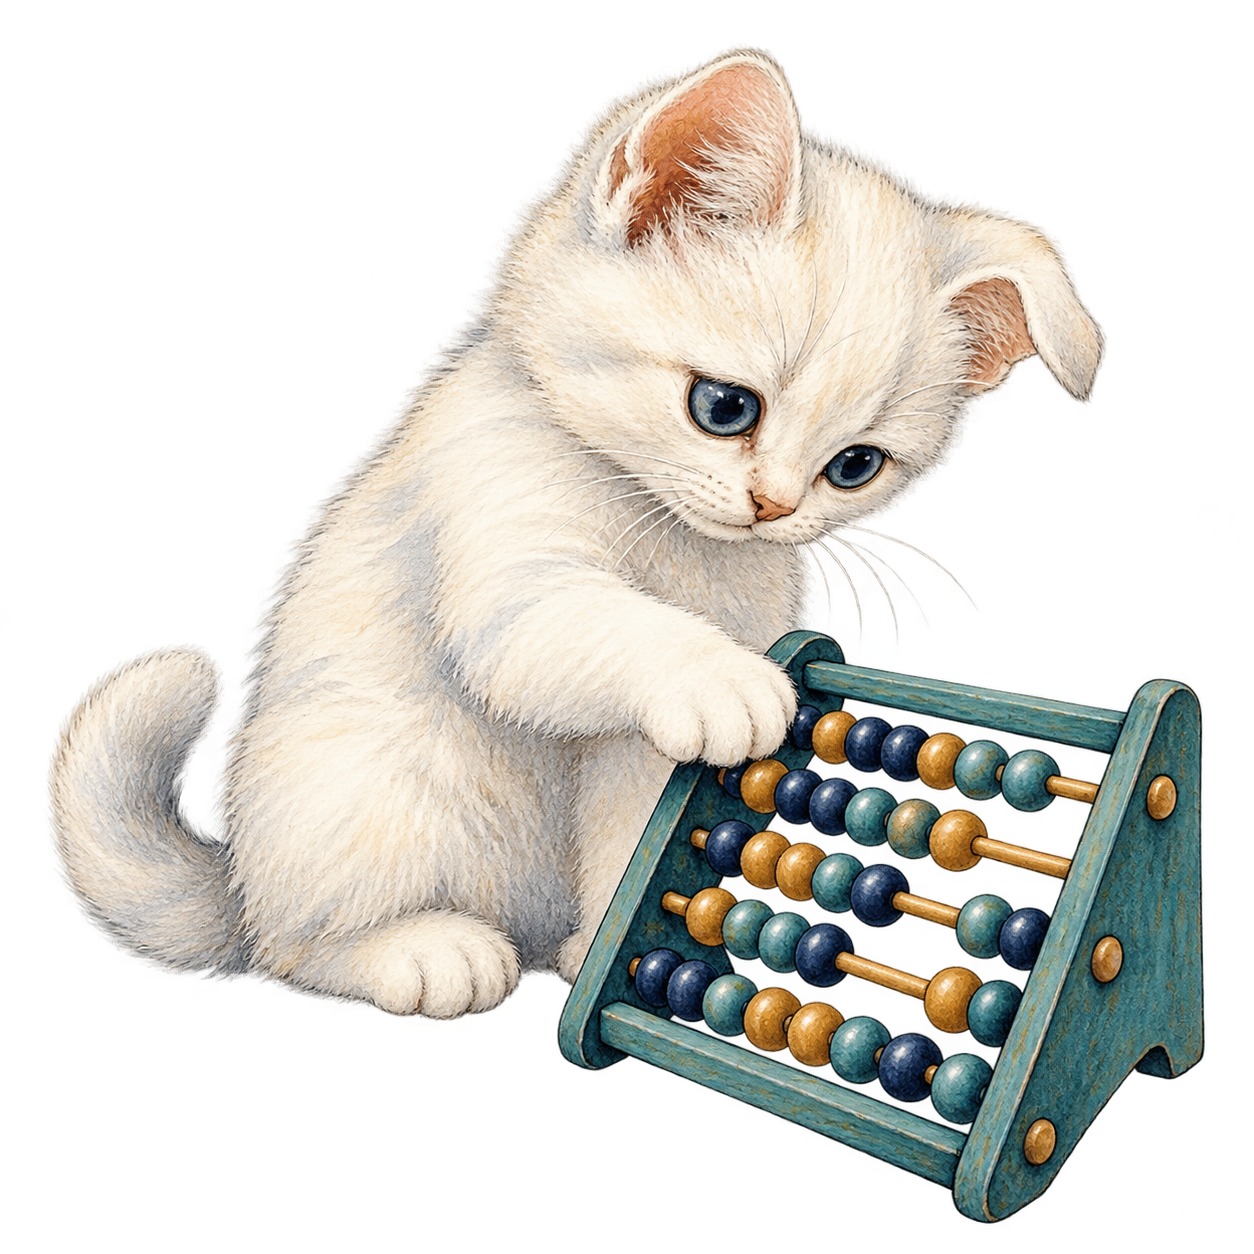
\includegraphics[width=54mm,height=58mm,keepaspectratio]{images/unique/art-306.png}
\label{catflow:306}
\end{wrapfigure}
\textbf{19.33.}\starmark{} {\small\itshape\href{https://www.apmo-official.org/static/problems/apmo1989_prb.pdf}{APMO, 1989, № 1}; перевод.}\par Пусть \(x_1,\ldots,x_n>0\), \(S=x_1+\cdots+x_n\). Докажи \[\prod_{i=1}^n(1+x_i)\le\sum_{k=0}^n\dfrac{S^k}{k!}.\]\par

\textbf{19.34.}\starmark{} {\small\itshape\href{https://www.apmo-official.org/static/problems/apmo1991_prb.pdf}{APMO, 1991, № 3}; перевод.}\par Положительные числа \(a_i,b_i\), \(1\le i\le n\), удовлетворяют \(\sum a_i=\sum b_i=S\). Докажи \[\sum_{i=1}^n\dfrac{a_i^2}{a_i+b_i}\ge\dfrac S2.\]\par
\par\WFclear\end{minipage}\end{lrbox}%
\ifdim\dimexpr\ht\CatFlowBox+\dp\CatFlowBox\relax<58mm\dp\CatFlowBox=\dimexpr58mm-\ht\CatFlowBox\relax\fi%
\noindent\usebox{\CatFlowBox}\par\addvspace{2pt}

\endgroup
